\chapter{Literature Survey}

Development of Wireless Sensor Network (WSN) is considered as one of the matured innovation in the field of electronics. The miniaturization of the components has allowed the user to explore applications in various fields such as health care, military applications, traffic control, monitoring, and data collection \cite{Khedo2017} \cite{Liu2017}. Out of all the applications, urban air quality monitoring has gained a lot of attention as it is one of the major issues faced by society today. While reviewing the related work, we found out that there are various methods used for understanding pollution. This could be classified into four based on literature as follows \cite{Yi2015} \cite{Pavani2017}.




%There are different approaches for measuring air pollution and this chapter gives an overview of the research work done for understanding this based on the medium for measurement. The popular mediums used for the measurement can be classified as below
 
\begin{enumerate}

    \item Vehicle-based sensor network
    \item Wearable sensor network
    \item Community sensor network
    \item Static sensor network

 \end{enumerate} 

 Further we will be highlighting the important research done in each of the above four categories and will be classifying to which category our work falls.

\section{Vehicle based sensor network (VSN)}

In recent times, the number of private vehicles on the road has increased in proportion to the increasing population around the globe \cite{Downs2004}. Even though the increase in the number of automobiles is one of the major factors that is contributing to the increase in pollution, certain researchers took this as a medium for measuring air pollution data. In this category of work, the vehicles (like buses or cars) are installed with a portable, low-cost sensor to obtain spatially resolved data. 
\par
%Portable and low-cost sensors are installed and attached to a vehicle like buses or cars in order to achieve a spatially resolved data. There have been an increasing number of mobile vehicles in urban areas. This was taken as a medium for obtaining air pollution data from the environment in cities. 
 One of the best ways to study the quality of air is by collecting fine-grained data also called \lq{micro-climate monitoring}\rq. However, with the existing monitoring system being bulky and expensive it is impossible to obtain spatially resolved data. To solve this issue, in 2009 a group of researchers used mobility as a method and proposed a vehicular wireless sensor network \cite{Hu2009} that measures the changes in concentration of a single pollutant measurement (Carbon Dioxide in this case) by mounting the sensor node onto a vehicle. The system is equipped with a Carbon Dioxide ($CO_2$) sensor, a Global System for Mobile (GSM) module, a GPS receiver, and a ZigBee module to create an intra-vehicular network. The collected data is transferred through GSM short messages to the server and is displayed on Google Maps for results. The architecture of the VSN is shown in the figure\ref{vsn}. 

 \begin{figure}[h!]
  \begin{center}
  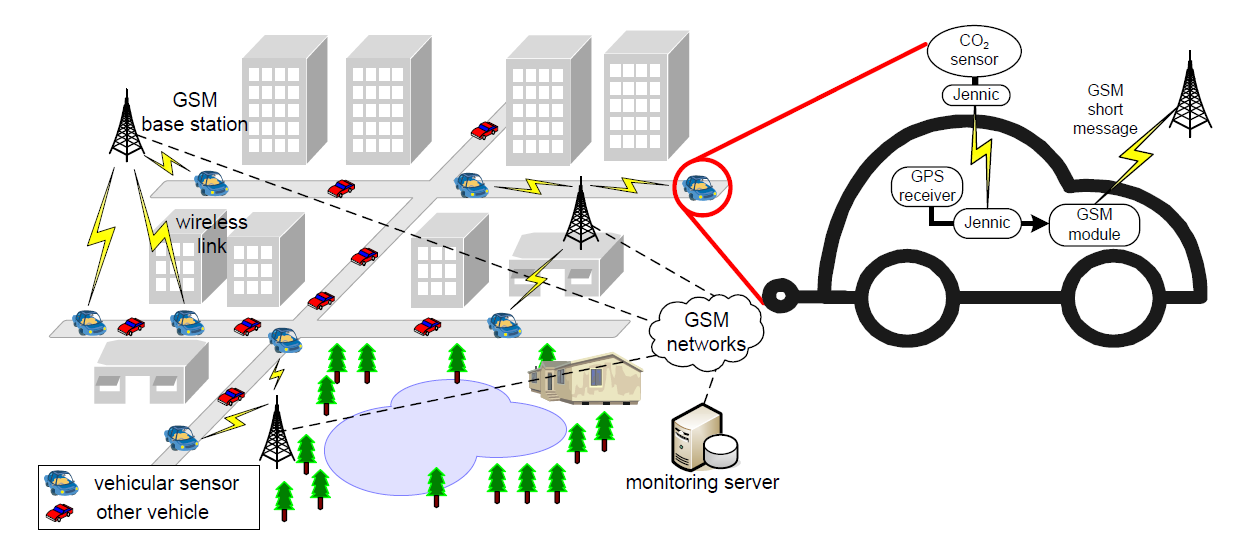
\includegraphics[scale=0.65]{./images/figure40.png}
  \end{center}
 
  \caption{Architecture of Vehicular based sensor network \cite{Hu2009}}
  
  \label{vsn}
\end{figure}
 
 This work faced two network-related drawbacks. Firstly there was a duplication of air pollution data as the number of vehicles in a given area changed dramatically from time to time and secondly, to reduce the data transfer in an area with many sensor nodes at the same time by exploiting opportunistic communication. These two problems were later addressed in 2011 \cite{Hu2011} by designing two message-efficient algorithms. The first algorithm works by dividing the sensing field into a fixed number of grids and each grid was allocated with a particular reporting rate which is called dynamic reporting rate to reduce communication overhead. The second algorithm allows the sensing nodes to communicate with each other and find out their reporting rate and opportunistically transfers the collected data. %The main area of the work revolved around data collection, optimization of the collected data, and concentrating only on one pollutant. The other issues like the quality and accuracy of the collected data, management and operations of wireless sensor networks were not given priority.



 %They also created a simulation model to verify the performance of the algorithm. The above two research work mainly focused on data collection, optimization of the collected data, and only revolved around one pollutant. The problems like calibration of sensors, visualization of data, checking the accuracy of the collected data, and management of the VSN was not taken care of.
\par

 Volgyesi et al. \cite{Volgyesi2008} proposed the Mobile Air Quality Monitoring Network (MAQUMON) that measured three pollutants, Ozone ($O_3$), Carbon Monoxide ($CO$), and Nitrogen Dioxide ($NO_2$). The air pollution system is mounted on a car and is powered by a Li-ion battery whose battery life is limited to a few hours. It is equipped with a GPS module for determining the location and the collected data is transferred to a laptop through a Bluetooth module. When the system is in coverage of a Wi-Fi network the collected data is transferred to a web server and visualized in sensor map web application in the form of contour maps. %However, the inability of representing instantaneous data is one of the main concerns with this system and also have failed to show the accuracy of collected data to the local system.


\par


The data collection that involves more frequent and spatially dense pollutant measurement is called a fine-grained approach. In \cite{Devarakonda2013}, the vehicular-based approach of measuring
fine-grained air quality in real-time was demonstrated. To increase the spatial density the study proposed two data collection models one for public transportation infrastructure and the other for a personal sensing device. A Mobile Sensing Box (MSB) was installed in public transit buses which contained the microcontroller (Arduino), sensors for measuring Particulate Matter ($PM$), Carbon Monoxide ($CO$), a GPS module and a cellular modem. The module was powered through the bus batteries and the collected data were transferred to a server and visualized using Google Fusion tables interfaces. In the second framing, a Personal Sensing Device (PSD) that included an air quality sensor was installed in cars and connected via Bluetooth to a smartphone. This gave the user information about the air quality while driving through a specific area.
The data obtained from both the framing models were compared using linear regression and the results showed a positive linear relationship between the data sets. Even though there was a high correlation seen between the two sets of data there was no comparison with the local reference data to understand the accuracy of the system.

\par

A similar technique of data collection like in \cite{Devarakonda2013} can be seen in wireless sensor deployment \cite{Saha2017} that proposed the idea of placing the sensor nodes in public transport buses to obtain real-time data of pollutants. The system here is divided into sensor node and sink node in which the former collects the data from the environment and the latter aggregates the data from the sensor node and transmits to a server via a long-range radio band. These sink nodes are either installed in a T-junctions or an X-junction of the city where most of the buses cross. The data is transferred at a regular interval of time and can be analyzed instantly. However, the paper did not discuss the collection of data and failed to provide the quality of collected data.



A research group from Japan, Shirai et.al \cite{Shirai2016} proposed an effective method to acquire air quality data in an urban areas in which the air pollution system has a sensing unit kept on a public vehicle like a garbage truck and garbage patrol vehicle which moves in and around the city. The main focus is on pollutants like Particulate Matter ($PM$), Carbon Monoxide ($CO$) and Sulphur Dioxide ($SO_2$), and is also aided with GPS module. To remotely monitor the sensing conditions and to check for maintenance, a control center tool has also been developed. It consists of a map that tracks the route of the vehicles and the sensor data acquired by each vehicle. A monitor was developed along with the system to send the users the collected data. It estimates the amount of pollution inhaled by the user like one in \cite{Devarakonda2013} which by acquiring the user's location from the mobile application and mapping it to the location-sensors value which has been already computed. It also considers the respiratory volume of the user to estimate the pollution inhalation.

Another mode of transportation that was taken for understanding the air quality was the public bicycle system. The bicycle borne sensor \cite{Xiang2016,Liu2015a} deploys a system equipped with an exhaust gas sensor, Particulate Matter ($PM$) sensor, GPS module, and a microprocessor. The system collects data along with the location from the GPS module and is stored in a micro storage chip. The system is powered with the help of Lithium polymer batteries. When the subscriber returns the bicycle to the dock station the data is transferred to the data center via the Bluetooth module and is then visualized using the 'Baidu' heat map.

In \cite{Zhi2017}, Unmanned Aerial Vehicle (UAV) is used as a medium to understand air quality.  In contrast to the work done in \cite{Hu2009,Hu2011,Volgyesi2008,Devarakonda2013,Shirai2016,Xiang2016,Liu2015a,Saha2017} this work focused on six different pollutants that contribute to Air Quality Index by mounting the sensor board on the flight. The flights are carried out in 30 days with 20 minutes of monitoring. Along with the sensor board, a smartphone is attached that collects data from the air sensor by establishing a Bluetooth connection. The collected data is transferred to air quality analysis software that will display the real-time monitoring value along with AQI value. 

The existing studies in this section show that collecting data using VSN supports micro-climate monitoring. The advantage of having spatially resolved data is that it helps to understand the trends of pollution in a better way. At the same time, the probability of having redundant data due to traffic congestion or duplication of data is high. Another concern is that there was no effort taken to understand the quality of data obtained. The main idea of deploying the system is to educate citizens and make them aware of the quality through the indexes. 
The efforts to calculate AQI or AQHI is not taken as a priority except in \cite{Zhi2017}. The representation of these indexes will make people aware of the air quality but most of the work in this category has failed to bridge the data gap.


\section{Wearable sensor network}


The individual effect of pollutants on health depends on the extent to which a person is exposed to the polluted environment. The understanding of the health effects could be achieved by observing the exposure-response relationship \cite{Dons2017} this will give an idea about the amount of pollutants inhaled by an individual. This could be achieved by using a wearable sensor which helps to understand the effects of individual impact when exposed to polluted air. Research was done in this section mainly focuses on improving the understanding of personal health and exposure to air pollution \cite{Hu2015}. One such development is Mypart \cite{Tian2016}  from the University of California, which is a wrist-worn particle sensor that measures particulate matter of 10 microns or less.  The design of MyPart is based on a traditional laser-based photodiode system with improvement in airflow to remove light leakage, integration of structural design and circuitry for ambient visualization, BLE transceiver for low power networking, and also a mobile application for visualization. Two main issues tackled by MyPart is accuracy and calibration of sensor which no existing consumer sensor has addressed.

Another related work is 'Eco-mini'\cite{Fletcher2015} which is a wearable stand-alone device for clinical use that measures Volatile Organic compounds (VOCs), sound level, air quality, temperature, and humidity values. This system is based on a low power microcontroller (Atmel Xmega 128k) and consists of a GPS module for position identifying and a Bluetooth module for data transfer. They modified the webserver which was developed on a simple javascript application. The next wearable work is 'citisense' \cite{Zappi2012} which is a system attached to a bag stripe which measures air pollutants like Nitrogen Dioxide ($NO_2$), Carbon Monoxide ($CO$), and Ozone  ($O_3$) along with environmental parameters such as temperature, humidity, and barometric pressure. The collected data from the sensor is processed by the microcontroller (ATMEGA1284p) and transfers the data using a Bluetooth module to a smartphone which does the data storing, analysis, and data aggregation. The collected data is then transferred to a back-end webserver from where the user can get a personalized view of their data. They also developed a citisense android application that runs on the smartphone.
 
In \cite{Kim2010}, the research group in the US developed an expressive T-shirt called 'WearAir' which indicates the measured Volatile Organic Compound (VOC) through expressive patterns. The T-shirt is designed with a metaphor of a car emitting gases with four vertical arrays of LEDs which shows different frequencies depending on the concentration of VOC gas in the surrounding. When the wearer is exposed to dense VOCs the LED will blink rapidly. 
The authors of \cite{Hu2014} developed a novel system consisting of several sensors that give real-time feedback on an individual's exposure dose. This consist of arm sensors, chest sensor or even wrist sensors which measures various pollutant concentration ($CO$ in this case) and transfers to an android or ios application via Bluetooth. They also calculate the inhaled dose of pollutants by calculating the volume of air inhaled into a person's lung per minute through an algorithm developed in \cite{Valli2013}. The inhaled dose of the pollutant was calculated and compared during various activities like jogging, bicycling, and driving.

 There are also wearable sensor projects initiated in Vancouver in association with the University of British Columbia like TZOA \cite{tzoa} that can be clipped to the clothing and measures the air quality. It mainly measures $PM$ values and display in an application. These devices decrease the gap between individual and their understanding of the polluted air. In NewYork a striking project named 'Aircasting'\cite{aircasting} provides the health and environment data using the android 'Aircasting app'. The 'Aircasting'\cite{Han2010} platform includes a palm-sized air quality monitor that measures $PM_{2.5}$, relative humidity, and temperature. The outside air is drawn through a sensing chamber and the particles are measured through the light scattering method. It also includes a LED wearable apparel named 'Air casting luminescence'\cite{Luminescence} that illuminates LEDs according to the obtained sensor measurement; varying from red for high intensity, then orange, then yellow, and finally green for low intensity. 
 
 The emergence of such wearables makes individuals be more cautious about their health and encouraged people to stay fit. At the same time, the public is not aware of these devices and does not prefer wearing T-shirts or carry a device for understanding the impact of pollution. Another issue to be focused on is the cost and stability of connection due to which the measured data values won't be able to visualize.



\section{Community sensor sensor}

The development of portable sensor devices has paved way for a novel paradigm for monitoring the pollution known as crowdsourcing or participatory sensing. This gives an opportunity for any citizen to collect data and transfer it to a common platform like a web interface. The collected data from the participants give a spatiotemporal view of the effect of pollution \cite{Kanhere2013}. In Sydney, a low-cost participatory system is deployed named 'Haze-watch' \cite{Sivaraman2013} for monitoring pollution in urban areas. In this, mobile sensor units were attached to vehicles, and collected data were transferred using Bluetooth to a mobile application which tags its location with date and time information. This data is then sent to a cloud-based server that stores data and applies interpolation models \cite{Liao2006} to generate Spatio-temporal estimates. Then using a web application the geo-referenced data is depicted as a contour map. 
\par
Intel has developed a prototype named 'Common Sense' \cite{Dutta2009} which is based on mobile participatory sensing \cite{Abdelzaher2007} that enables citizens to collect relevant data and involves in the decision making process. The system includes a handheld device that measures a couple of pollutants and uploads the value for visualization over the web using Bluetooth or GPRS radios. This work was further tested by deploying it on a municipal fleet of street sweepers in the city of San Francisco \cite{Aoki2008}. Another community-driven sensing developed is 'OpenSense' \cite{Aberer2010} which focuses on the utility of data by giving an idea about how the data collected from sensors needs to be consumed. They have provided two use-cases first one is smart healthcare which by giving alerts on identifying the pollution-induced diseases (like asthma, particle allergies, etc.) and next is urban planning by identifying polluted areas and identifying alternative routes. The system is deployed on mobile vehicles and stationary stations in Switzerland and the collected data is pipelined to a Global Sensor Network (GSN) from where the streamed data is processed and represented. In \cite{Hasenfratz2012} an outdoor participatory monitor was introduced called 'GasMobile' by connecting a low-cost ozone sensor to an android smartphone. The collected data from the sensor is transferred to the phone and from which it is visualized using an application as well as a webserver. They have also implemented calibration procedures to the low-cost sensors and the work claims to have high accuracy when compared to static measurement. The above-mentioned research work in 'OpenSense' and 'GasMobile' have made an opening for further participatory sensing research in Switzerland supported by Samsung called 'Exposuresense' \cite{Predic2013} that monitors user activities like walking, running, etc., from smartphones and understanding their exposure from obtaining data from the already installed 'OpenSense' and 'GasMobile'. Their main idea here is to make use of the available smartphone for next-generation healthcare.
\par
The growth of the Micro-Electro-Mechanical System (MEMS) and Wireless Sensor Network (WSN) have made difference in the way how data is collected and understood from the physical world. 'G-Sense' \cite{Perez2010}, for Global-Sense, is a work initiated from the University of Florida in which they combine features of sensing platform applications like Location-Based Services (LBS) for tracking and location identification, Participatory Sensing (PS) for determining pollution index, and other environmental data, and Human-Centric Sensing (HCS) for health-related data for a specific group of users. The sensors collect the data and sends to a first-level integrator where all the data gets collected and from there using a data transport network it is transferred to the server that stores and performs data processing. It is from the server where the data visualization takes place which reports the data. Later there was another work which is considered to be the subset of G-Sense and named as 'P-Sense' \cite{Mendez2011} or Pollution-Sense. The architecture of this system is based on G-Sense in which external sensors are integrated into an Arduino development board. In this, the data collection is based on Participatory Sensing (PS) and the goal here is to provide government officials, doctors, and community developers with data so as to get a deeper understanding. They have also pointed out the research-oriented challenges that need to be addressed when building a community networked system like security, privacy, data visualization, and working towards achieving them. 

The work discussed in this category seems to be more promising but at the same time the quality of data obtained, getting public involvement for data collection, and privacy issues \cite{Yi2015} are a few challenges researchers are trying to work towards it. The cost of maintenance in such a community network in case of any damage is a crucial factor.



\section{Static sensor network}

 In this category, the system is kept at a fixed location like traffic lights, street lights or any planned areas \cite{Pavani2017} which collects the pollutant values and transfers it to a visualization platform where the users can view it instantly. These systems are inexpensive and can be easily replicated or replaced. The system can be used for measuring either indoor or outdoor pollutants. The already existing station based environmental monitoring system is complex, bulky, and expensive; hence there is a need to develop a portable and low-cost environmental monitoring system. There is various noticeable research work done under this category and I have briefed relevant ones.
 \par
  The Integrated Environmental Monitoring System (IEMS)\cite{Wong2014}, integrates different environmental detection sensors in a single system, and data from this system is used for processing and visualization. IEMS consist of Integrated Environmental Monitoring Device (IEMD) which consists of Microcontroller units, sensors, wireless communication module. They developed the Handheld Remote Control Panel (RCP) for the system which is an android application that acts as an interface for the device control and handles the data exchange between IEMD and Web Server. Finally, the webserver that provides real-time data visualization and data analysis. These systems were placed on bus stops, bridges, and even in the construction sites. Another research team from Mauritius developed a Wireless Sensor Network Air Pollution Monitoring System (WAPMS) \cite{K.Khedo2010} that designed a data regression algorithm named Recursive Converging Quartiles (RCQ) to remove duplicate data and then calculate AQI values. The array of sensor nodes collects the pollutant data and transfers it to cluster heads where the RCQ is applied to improve efficiency and alleviate the congestion problem. From the cluster head, the data is sent to the server and represented using line graphs for each area.

'AirSense'\cite{Fang2016} is an excellent approach to assess indoor air quality. The author tries to introduce the idea of indoor air quality to the society by proposing a system which measures indoor pollutants. The system works through electronic sensors that are coupled to an Arduino (processing unit). The system not only extracts the data but also provides its users with very effective visualization and analysis of the data. The researchers have done an excellent job of developing this robust system that would sense the pollution and provide education and awareness among the users. This system has made use of some machine learning algorithms to predict the pollution sources and forecast their behaviour so as to provide intelligence to the system. 
The system has also got a smartphone application that gives the users a very effective interface for visualizations and understanding of the data. In \cite{Liu2017} a different group of researchers from China developed the system 'Air-Sense' to monitor and predict the quality of air based on the ZigBee network. The system uses four different types of sensors, respectively are humidity, temperature, $PM_{2.5}$, Total Volatile Organic Compound (TVOC includes the general organic gases), and a ZigBee trans-receiver for communication with network nodes. The prototype is tested for different areas in the house. It collects data in real-time and using Bayesian mathematical statistics it predicts how accurate is the collected value to the standard value predicted by WHO. 
\par

Another static work that focuses on indoor air quality is demonstrated in \cite{Firdhous2017} in which the main focus is to understand the pollution in an office environment where the pollution is triggered by the electronic devices and machines. In this, the primary pollutant measured is ozone which is mainly emitted from a photocopier machine. The system is designed into different nodes where the sensing node contains the Arduino which processes which collects the data from the ozone sensor. The measured data is transferred through a Bluetooth link to a gateway node from where the data is formatted as IP packets and forwarded over the Ethernet network to the processing node. The data is saved in the database and using a 2D graph the concentration gets visualized. A research group from Harvard University developed a wireless networking testbed called as 'CitySense' \cite{Murty2008} in which multiple environmental sensors are attached to street lights. These sensors were deployed in Cambridge and data was uploaded to the server using mesh networking like RoofNet \cite{Bicket2005}, TFA \cite{Camp2006}, and CUWin \cite{cuwin2006}. Using a Web-based interface the data can be pulled from the server and made available to end-users. The main feature of this research work is that the sensor nodes are powered from street lights and there is no constraint about long battery life.
\par
Liu J.H. et al \cite{Liu2011} developed a micro-scaled air quality monitoring system for understanding the $CO$ emission from vehicles by integrating the sensor nodes with a gateway. The data collected from the sensor is transferred to the gateway using a ZigBee communication link and from here meteorological data and collected sensor data are forwarded to a central system through short message service via GSM. This centralized control system is supervised by the LabVIEW \cite{INSTRUMENTS2013} programming which helps in storing the data into the MySQL database. They deployed the system on the main roads of Taipei city and obtained accurate values of pollutant concentration.

Our research work falls under a static sensor network in which we have tried to integrate a system that measures all the major pollutants in the city of Prince George and also providing AQHI values. Unlike the other system mentioned in the literature, our main focus is to give  user-specific data for a better understanding of pollution. We have categorized the users into three; layman, data scientist and the officials. We have also tried to implement a calibration procedure to ensure the quality of data. 

 \section{Summary}

 In this chapter, the research done in the sensor network for understanding the air quality is categorized into four. We went through the system which is attached to a vehicle for understanding the pollutant concentration and gets categorized as a vehicular sensor network. This category provides great mobility but at the same time, the accumulation of redundant data is high.
 The next category we mentioned is the sensors that could be worn or attached to a person. This gives a better understanding of the individual health effects of the pollutant and also the amount of pollutant inhaled. The work under this category has not gained a lot of attention as it demands the individual to carry the device. 
Participatory sensing is the next category in which the citizens perform the collection of data and it gets transferred to a common platform. Although the work done in this is more promising it faces challenges like privacy, data quality, and maintenance cost. The final category is in which the system is placed at a planned area and called as a static sensor network. Our research work falls under this section and we focus not just on collecting pollutant value but also on making an effective visualization to reduce the data gap for users.